\message{ !name(cbv8.tex)}%&latex
\documentclass[10pt,fleqn]{article} 

\pdfoutput=1

\addtolength{\oddsidemargin}{-.875in}
\addtolength{\evensidemargin}{-.875in} \addtolength{\textwidth}{1.75in}

\addtolength{\topmargin}{-.875in} \addtolength{\textheight}{1.75in}

\openup 1em

%macro for commenting
\usepackage{color}

\newcommand{\leo}[1]{{\color{blue}{#1}}}
\newcommand{\alex}[1]{{\color{red}{Alex: #1}}}

% \newcommand{\Xbeta}{ X_i \theta}
\newcommand{\xbeta}{ x_i \beta} \newcommand{\xtheta}{ x_i \theta}
% \newcommand{\xbetaij}{ x_{ij}^T \theta}
\newcommand{\sgamma}{s_{ij}^T\gamma_i} \newcommand{\core}{\textbf{CORE}}

\usepackage[round]{natbib}

\usepackage{rotating} \usepackage{graphicx} \usepackage{subcaption}

\usepackage{float} \usepackage{bbm}

\usepackage{amsthm,amsmath, amssymb} \usepackage{mathrsfs}
\usepackage{subcaption}
\usepackage[normalem]{ulem}
%\usepackage{nicefrac}

\usepackage{tikz}

\newtheorem{theorem}{Theorem} \newtheorem{lemma}{Lemma}
\newtheorem{corollary}{Corollary} \newtheorem{remark}{Remark}
\newtheorem{example}{Example} \newtheorem*{Hausdorff_def}{Definition -
Hausdorff Measure}


\usepackage{algorithm} \usepackage{algpseudocode} \usepackage{array}

%\usepackage{mhequ}
\newcommand{\be}{\begin{equation}\begin{aligned} }
\newcommand{\ee}{\end{aligned}\end{equation} }
\newcommand{\bb}[1]{\mathbb{#1}} \newcommand{\mc}[1]{\mathcal{#1}}
\DeclareMathOperator{\Binom}{Binomial} \DeclareMathOperator{\No}{No}
\DeclareMathOperator{\PG}{PG} \DeclareMathOperator{\IG}{Inverse-Gamma}
\DeclareMathOperator{\Ga}{Gamma} \DeclareMathOperator{\Bern}{Bernoulli}
\DeclareMathOperator{\U}{Uniform} \DeclareMathOperator{\Poi}{Poisson}
\DeclareMathOperator{\NB}{NB} \DeclareMathOperator{\cov}{cov}
\DeclareMathOperator{\var}{var} \DeclareMathOperator{\diag}{diag}
\DeclareMathOperator{\Diag}{Diag}
\newcommand{\KL}[2]{\textnormal{KL}\left(#1 \parallel #2\right)}
\DeclareMathOperator{\1}{\mathbbm{1}} \DeclareMathOperator{\bigO}{\mc O}
\newcommand{\dt}{\epsilon} % Stepsize of leapfrog
\newcommand{\mass}{M} %Mass matrix 
\newcommand{\hess}{\mathbf{H}} % Hessian notation.



\thispagestyle{empty} \baselineskip=28pt

\title{\textbf{Bayesian constraint relaxation}}

\author{Leo L Duan, Alexander L Young, Akihiko Nishimura, David B Dunson} 

\date{}
\begin{document}

\message{ !name(cbv8.tex) !offset(301) }
\subsubsection{Constrained Space with Zero Measure}
\label{SEC:Zero_Measure_Methods}

We now consider the more challenging case in which $\mathcal{D}$ is a measure
zero subset of $\mathcal{R}$ with respect to $\mu_{\mc R}$, \leo{the Lesbesgue
measure}. This introduces challenges in associating the constrained $\pi_{\mc
D}(\theta \mid Y)$ with an unconstrained density $\mathcal{L}(\theta; Y)\pi_{\mc
R}(\theta)$, as simple re-normalization is invalid. For example, consider the
constrained space $\mc D = \{\theta: \theta_1+\theta_2=1\}$, with $\pi_{\mc R} =
1\{\theta_1 \in (0,1),\theta_2 \in (0,1)\}.$ Then, $\pi_{\mc R}(\mc D)=0$ and
the constraint relaxed posterior (\ref{EQ:relaxedDensityPosMeasure}) is
undefined. One possibility is to \leo{focus on lower dimension by replacing
  $(\theta_1,\theta_2)$
  with $(\theta_1,1-\theta_1)$, deriving the appropriate density.
}
% reparameterize, replacing $(\theta_1,\theta_2)$ with a single $\theta$ to avoid these measurability
%problems. However, it is not clear how to include constraint relaxation when
%reparameterizing to a lower dimension.
Alternatively, one can `thicken' the
space to $\mc D_{\epsilon} = \{\theta: \theta_1+\theta_2\in
(1-\epsilon,1+\epsilon)\}$ in defining the relaxed posterior density,
\leo{without having to focus on lower dimension}. Building
on this intuition, \leo{the focus on the lower dimension corresponds to a geometric measure
%theory concept known as a Hausdorff measure, and latter corresponds to a Lesbesgue}
%we will formalize the CORE posterior via a geometric measure
%theory concept known as a Hausdorff measure.

For constructing a valid constrained density, we restrict
ourselves to cases in which $\mathcal{D}$ can be represented implicitly
as the unique solution set of a consistent system of equations $\{v_j(\theta) =
0\}_{j=1}^s$, so that $\mathcal{D} =\{\theta : v_j(\theta) =0, \, j =
1, \dots,s\}$ is an $(r-s)$-dimensional subspace of $\mc R$. This is equivalent to using the distance $\|v_\mathcal{D}(\theta)\|=\sum_j \| v_j(\theta)\|=0$, with $ \| v_j(\theta)\|$ chosen as described in 
Section 2.1.
%provided the space formed satisfy the $(r-s)$-dimensionality requirement.

While $\mathcal{D}$ has zero $r$-dimensional Lesbesgue measure, corresponding to zero volume within $\mathcal{R}$, it has positive $(r-s)$-dimensional surface area.  This surface area corresponds to the 
$(r-s)$-dimensional Hausdorff measure, denoted by $\bar{\mathcal{H}}^{(r-s)}$. Taking the Hausdorff measure of a Borel subset of $\mc D$ and normalizing  it by $\bar{\mathcal{H}}^{(r-s)}(\mc D)$ yields a valid probability in the constrained space. Additional technical details will be provided in Section 3.  Using the Hausdorff measure to define the sharply constrained posterior, we let 
$$\pi_{\mc D}(\theta \mid Y) = \dfrac{
{\mathcal{L}(\theta;Y)\pi_\mathcal{R}(\theta)}{J^{-1}(v_\mathcal{D}(\theta))
\mathbbm{1}_{\mc D}(\theta)
}
} {\int_\mathcal{D}
{\mathcal{L}(\theta;Y)\pi_\mathcal{R}(\theta)}{J^{-1}(v_\mathcal{D}(\theta))}
d\bar{\mathcal{H}}^{(r-s)}(\theta)} \propto
{\mathcal{L}(\theta;Y)\pi_\mathcal{R}(\theta)}{J^{-1}(v_\mathcal{D}(\theta))
\mathbbm{1}_{\mc D}(\theta)
},
$$
defined with respect to $\bar{\mathcal{H}}^{(r-s)}$, where $J(v_\mathcal{D}(\theta)) =
\sqrt{(Dv_\mathcal{D})'(Dv_\mathcal{D})}$ is the Jacobian
of $v_\mathcal{D}$, which we assume is positive.   
%Sometimes it is possible to reparameterize $(r-s)-$ dimensional Hausdorff density (with $r$ parameters) and convert to a $(r-s)-$ parameter Lesbesgue density, as more commonly seen in statistical literature; but such reparameterization may not exist.  NOTE: this is unclear.  you can't reparameterize a density with r-s parameters to r parameters.

As in the positive measure case, to relax the constraint, we replace the
indicator function with an exponential function of $\|v(\theta)\|$, adding
support for  $\|v(\theta)\|>0$.  This expanded support now has a 
Lesbesgue measure

$$
{\int_{\mc X}
\bigg[ \int_{ \{\theta:v(\theta)=x\} \cap \mc R }
{\mathcal{L}(\theta;Y)\pi_\mathcal{R}(\theta)}{J^{-1}(v_\mathcal{D}(\theta))
)}
d\bar{\mathcal{H}}^{(r-s)}(\theta) \bigg]     \exp(-{\lambda^{-1}}\|x\|)    dx
},
$$
where $\mc X$ is the range of $v_{\mc D}(\theta)$. This measure is computed by first calculating the ``surface area'' of each slice
$\{\theta:v_{\mc D}(\theta)=x\}$ (inner integral) and then integrate out $x$ with an exponential
prior (outer integral). For this measure to be positive and finite, we impose a
truncation on $\mc X$, such that the inner integral is finite and positive
almost everywhere. This is equivalent to requiring each subspace defined
by $\{\theta:v_{\mc D}(\theta)=x\}$  to have the same dimension $(r-s)$ almost
everywhere in $\mc X$.
%Effectively, this truncation limits the expanded support
                       %of $\theta$ from $\mc R$ to the pre-image $v^{-1}(\mc X)$.

From now on, we use an indicator function $\mathbbm{1}_{\mc X}(.)$ to represent the truncation.
For a Borel subset $\mc F \subset \mc R$, we can obtain its normalized measure

\begin{equation}
\begin{aligned}
\int_{\mc F} \tilde{\pi}_\lambda(\theta) d \mu(\theta)= & \frac{\int
\bigg[ \int_{ \{\theta:v(\theta)=x\}\cap \mc F }
{\mathcal{L}(\theta;Y)\pi_\mathcal{R}(\theta)}{J^{-1}(v_\mathcal{D}(\theta))
}
d\bar{\mathcal{H}}^{(r-s)}(\theta) \bigg]  \exp(-{\lambda^{-1}}\|x\|) \mathbbm{1}_{\mc X}(x) dx
}
{\int\bigg[ \int_{ \{\theta:v(\theta)=x\} \cap \mc R}
{\mathcal{L}(\theta;Y)\pi_\mathcal{R}(\theta)}{J^{-1}(v_\mathcal{D}(\theta))
}
d\bar{\mathcal{H}}^{(r-s)}(\theta) \bigg]     \exp(-{\lambda^{-1}}\|x\|)   \mathbbm{1}_{\mc X}(x) dx
},
\end{aligned}
\end{equation}

When $\mc X$ is the Lipschitz image of a bounded subset in $\mc R$, i.e. $r$-rectifiable, the double integral  can be further simplified to a single Lesbesgue integral \citep{federer2014geometric}.

%This allows us to define the relaxed posterior as a density with respect to Lesbesgue measure, with this density assigning the following probability to the set $\mc F$: 

\begin{equation}
\begin{aligned}
\int_{\mc F} \tilde{\pi}_\lambda(\theta) d \mu(\theta) 
= & \frac{\int_\mathcal{F} \mathcal{L}(\theta;Y)
\pi_\mathcal{R}(\theta)\exp\bigg(-\frac{1}{\lambda}\|v_\mathcal{D}(\theta)\|\bigg)
\mathbbm{1}_{\mc X}(v(\theta)) d\mu_\mathcal{R}(\theta)}
{\int_\mathcal{R} \mathcal{L}(\theta;Y)
\pi_\mathcal{R}(\theta)\exp\bigg(-\frac{1}{\lambda}\|v_\mathcal{D}(\theta)\|\bigg)
\mathbbm{1}_{\mc X}(v(\theta)) d\mu_\mathcal{R}(\theta)}.
\end{aligned}
\end{equation}

Omitting the integral over
$\mc F$, this reduces to a constraint relaxed density:
\begin{equation}
\begin{split}
\label{EQ:relaxedDensityZeroMeasure}
\tilde{\pi}_\lambda(\theta)  & \propto \mathcal{L}(\theta;Y)
\pi_\mathcal{R}(\theta)\exp\bigg(-\frac{1}{\lambda}\|v_\mathcal{D}(\theta)\|\bigg)
\mathbbm{1}_{\mc X}(v(\theta)),
\end{split}
\end{equation}
which is defined with respect to $\mu_{\mc R}$. Note the remarkable similarity to the relaxed density in the positive measure case, except for a more restricted suitable range of  $v_{\mc D}(\theta)$.

For this relaxation, we again address the two important questions regarding its relationship to sharply constrained density and its limitations. First, the relaxed density no longer converges pointwise to the sharply constrained one, as they correspond to two different types of measure. Nevertheless, as $\lambda\to 0$, the relaxed measure concentrates to an arbitrarily small layer around the constrained space. Second, there are several limitations imposed on $\mc D$, $v(\theta)$ and $\mc X$, such as the dimensionality and rectifiability. However, this still include a large variety of constrained spaces, such as compact manifolds embedded in Euclidean space via Lipschitz functions (e.g. orthonormal space).
 More details will be discussed in the theory section. 

\textbf{Example: Support expansion near a curved torus}


For now, we consider a curved torus

$$\mc D= \big\{\theta: (\theta_1,\theta_2,\theta_3) = \big(
(1+ 0.5 \cos\alpha_1) \cos\alpha_2, (1+ 0.5\cos\alpha_1) \sin\alpha_2,0.5 \sin\alpha_1\big), (\alpha_1,\alpha_2)\in [0,2\pi)^2 \big\}.$$ 

As the intrinsic dimension is $2$ hence
 the $3$-dimensional Lesbesgue measure $\mu_{\mc R}(\mc D)=0$, with  $\mc R$ a compact $3$-dimensional Euclidean subspace. \cite{diaconis2013manifold} previously considered a uniform Hausdorff density $\pi_{\mc D }(\theta \mid Y) \propto 1$ over this compact manifold and utilized the transformed Lesbesgue density based on $(\alpha_1,\alpha_2)$ for sampling within the manifold.

We now consider a different task by considering a relaxed distribution near the manifold. It is intuitive to consider type-I distance to $\mc D$, with

$$v(\theta) =\|v(\theta)\|=\underset{  (\alpha_1,\alpha_2)\in [0,2\pi)^2}{\inf} \| (\theta_1-(1+ 0.5\cos\alpha_1) \cos\alpha_2 ,\theta_2 -  (1+ 0.5\cos\alpha_1) \sin\alpha_2,\theta_3
- 0.5\sin\alpha_1)\|_2.$$

We obtained a relaxed density:
$$\tilde\pi_{\lambda}(\theta) \propto {J(v_\mathcal{D}(\theta))\exp(-\lambda^{-1}\|v(\theta)\|)}$$
which is with respect to $3$-dimensional Lesbesgue measure. Note $v(\theta)$ and $J(v_\mathcal{D}(\theta))$ do not have closed-form,
fortunately, they can be numerically approximated by automatic optimization and differentiation tools. Figure~\ref{fig:torus}
plots the random samples from constraint relaxed posteriors
under two different values of $\lambda$, corresponding to different degrees of relaxation. The samples
were obtained using random walk Monte Carlo.


\begin{figure}[h]
\begin{subfigure}[b]{1\textwidth}
 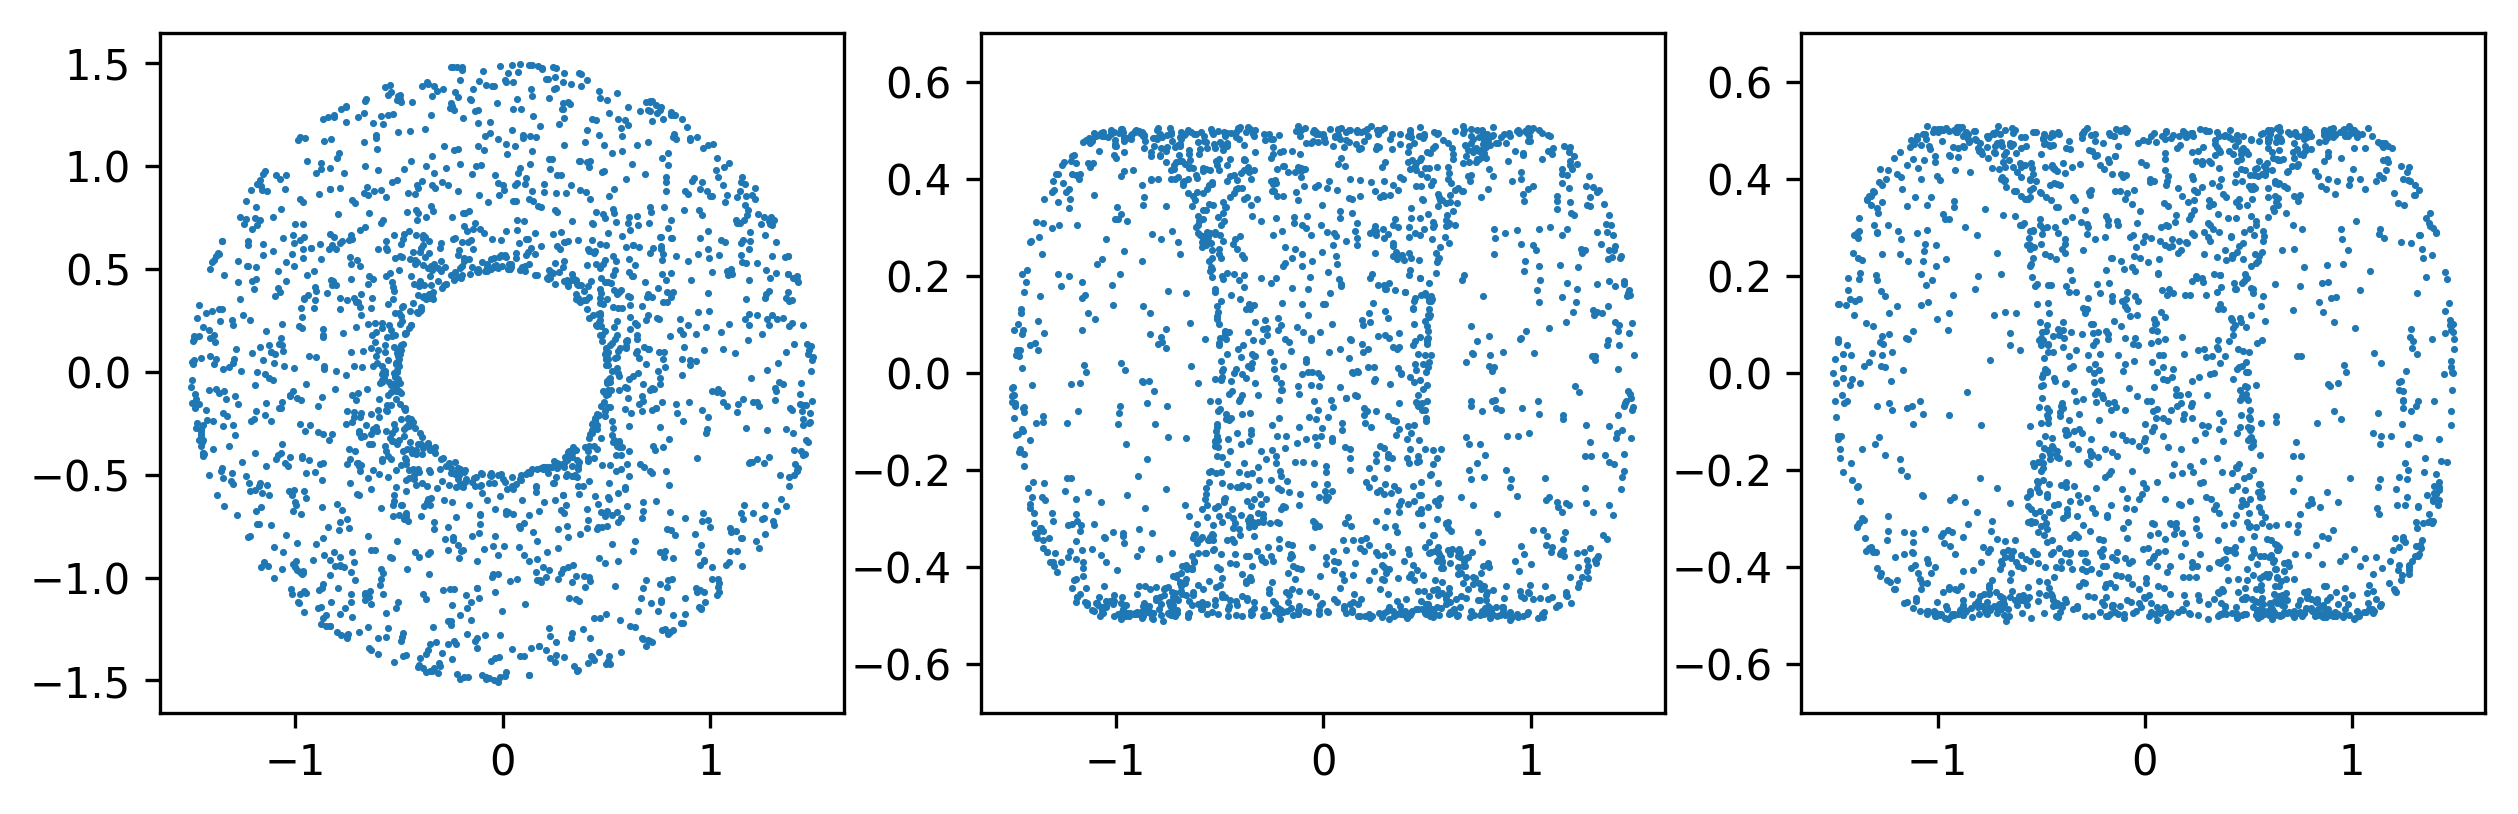
\includegraphics[width=1\textwidth]{torus_001.png}
 \caption{Constraint relaxed posterior with $\lambda
 = 0.01$}
\end{subfigure}
\begin{subfigure}[b]{1\textwidth}
 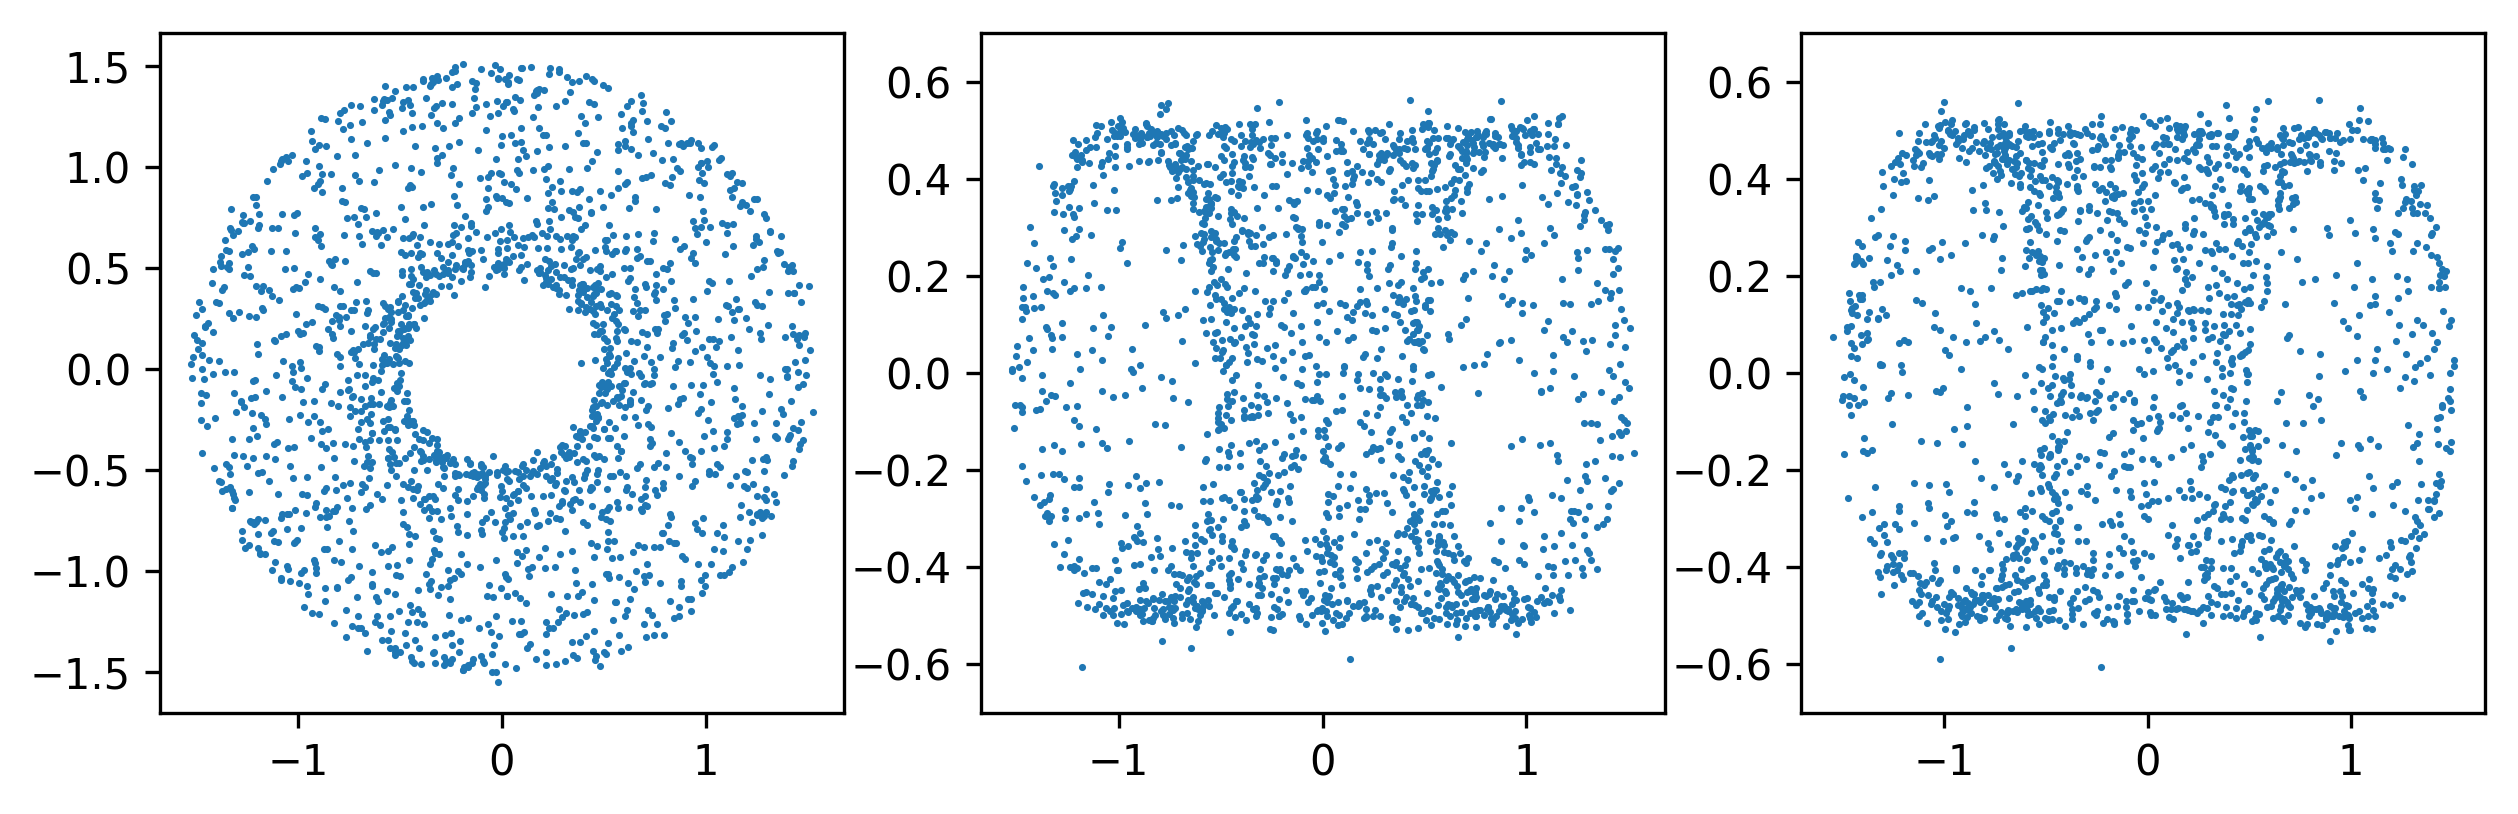
\includegraphics[width=1\textwidth]{torus_005.png}
 \caption{Constraint relaxed posterior with $\lambda
 = 0.1$}
\end{subfigure}
 \caption{Support expansion near a curved torus. Small $\lambda$ controls the samples to be very close to the manifold (upper panel), while large $\lambda$ adds support farther away from the constrained space (lower panel). Both densities correspond to more conventional Lesbesgue measure, instead of Hausdorff measure.
 \label{fig:torus}}
\end{figure}




\message{ !name(cbv8.tex) !offset(1224) }

\end{document}


